\documentclass[11pt]{article}
\usepackage[margin=1in]{geometry}
\usepackage{graphicx}
\usepackage{booktabs}
\usepackage{multirow}
\usepackage{longtable}
\usepackage{array}
\usepackage{float}
\usepackage{hyperref}
\usepackage{setspace}
\doublespacing

\title{Integrated cross-tribe phenotypic, behavioral, and dermatoglyphic profiling from community survey workbooks}
\author{Sweta Nidhi}
\date{}

\begin{document}
\maketitle

\begin{abstract}
Population-scale profiling of underserved tribal communities is often fragmented across administrative, anthropometric, and biosample spreadsheets, limiting integrated interpretation. We present a reproducible analytical pipeline for two tribe-level datasets (Nirankal and Virnoda) represented across roster, anthropometric, questionnaire, and fingerprint-hair sheets. The framework harmonizes schema inconsistencies, quantifies missingness, and performs multi-layer inference across demographic, body-composition, lifestyle, and dermatoglyphic dimensions. Statistical inference combines Mann-Whitney U testing, chi-square association testing, effect-size estimation (Cohen's $d$, Cliff's delta, Cramer's $V$), and false-discovery-rate control. Pattern discovery layers include principal component analysis and bilateral fingerprint symmetry metrics. Across 188 roster entries, Virnoda showed consistently higher central tendency for BMI and most body-circumference variables, but with predominantly small standardized effect sizes. Behavioral divergence was strongest for tobacco-use responses. Dermatoglyphic signatures revealed shared dominant classes (W, UL, PA) but markedly different repertoire diversity (Shannon entropy 3.205 in Nirankal versus 2.179 in Virnoda). These findings illustrate that tribe-level differences are best represented as multivariate profile shifts rather than single-variable contrasts.
\end{abstract}

\section{Introduction}
Indigenous and tribal populations are often analyzed through narrow, single-domain snapshots, while real-world survey operations generate richer but structurally heterogeneous data streams spanning family rosters, anthropometry, questionnaire responses, and biological descriptors. This disconnect between data collection breadth and analytic integration can obscure meaningful cross-group structure. Robust statistical synthesis requires careful harmonization, explicit treatment of missingness, and effect-size-centric inference rather than reliance on $p$-values alone.

This study integrates two tribe workbooks (Nirankal and Virnoda) into a unified analytical framework. Our goals are to quantify cross-tribe commonalities and divergences across demographic, anthropometric, behavioral, and dermatoglyphic layers; report both statistical significance and practical effect sizes; benchmark data quality and missingness explicitly; and provide a reproducible analysis framework.

\section{Contributions}
This work contributes a reproducible multi-sheet harmonization pipeline, an integrated inferential stack combining non-parametric and categorical tests with effect-size and FDR adjustment, and a dermatoglyphic diversity and symmetry layer.

\section{Methods}
We analyzed two workbooks: Nirankal and Virnoda. Sheets were mapped to four analytical domains: roster, measurements, questionnaire, and fingerprint-hair. Column-level normalization addressed common operational inconsistencies such as sheet-name variation, mixed-case labels, and numeric coercion. All-empty rows were removed. Age values were converted to numeric where possible. Categorical values were normalized to uppercase and whitespace-cleaned. Fingerprint records were converted to long format for per-code composition statistics. Statistical procedures included Mann-Whitney U tests, chi-square tests, Cohen's $d$, Cliff's delta, Cramer's $V$, and Benjamini-Hochberg correction. Pattern discovery included PCA on standardized anthropometric variables and Shannon entropy of fingerprint-code distributions.

\begin{figure}[H]
\centering
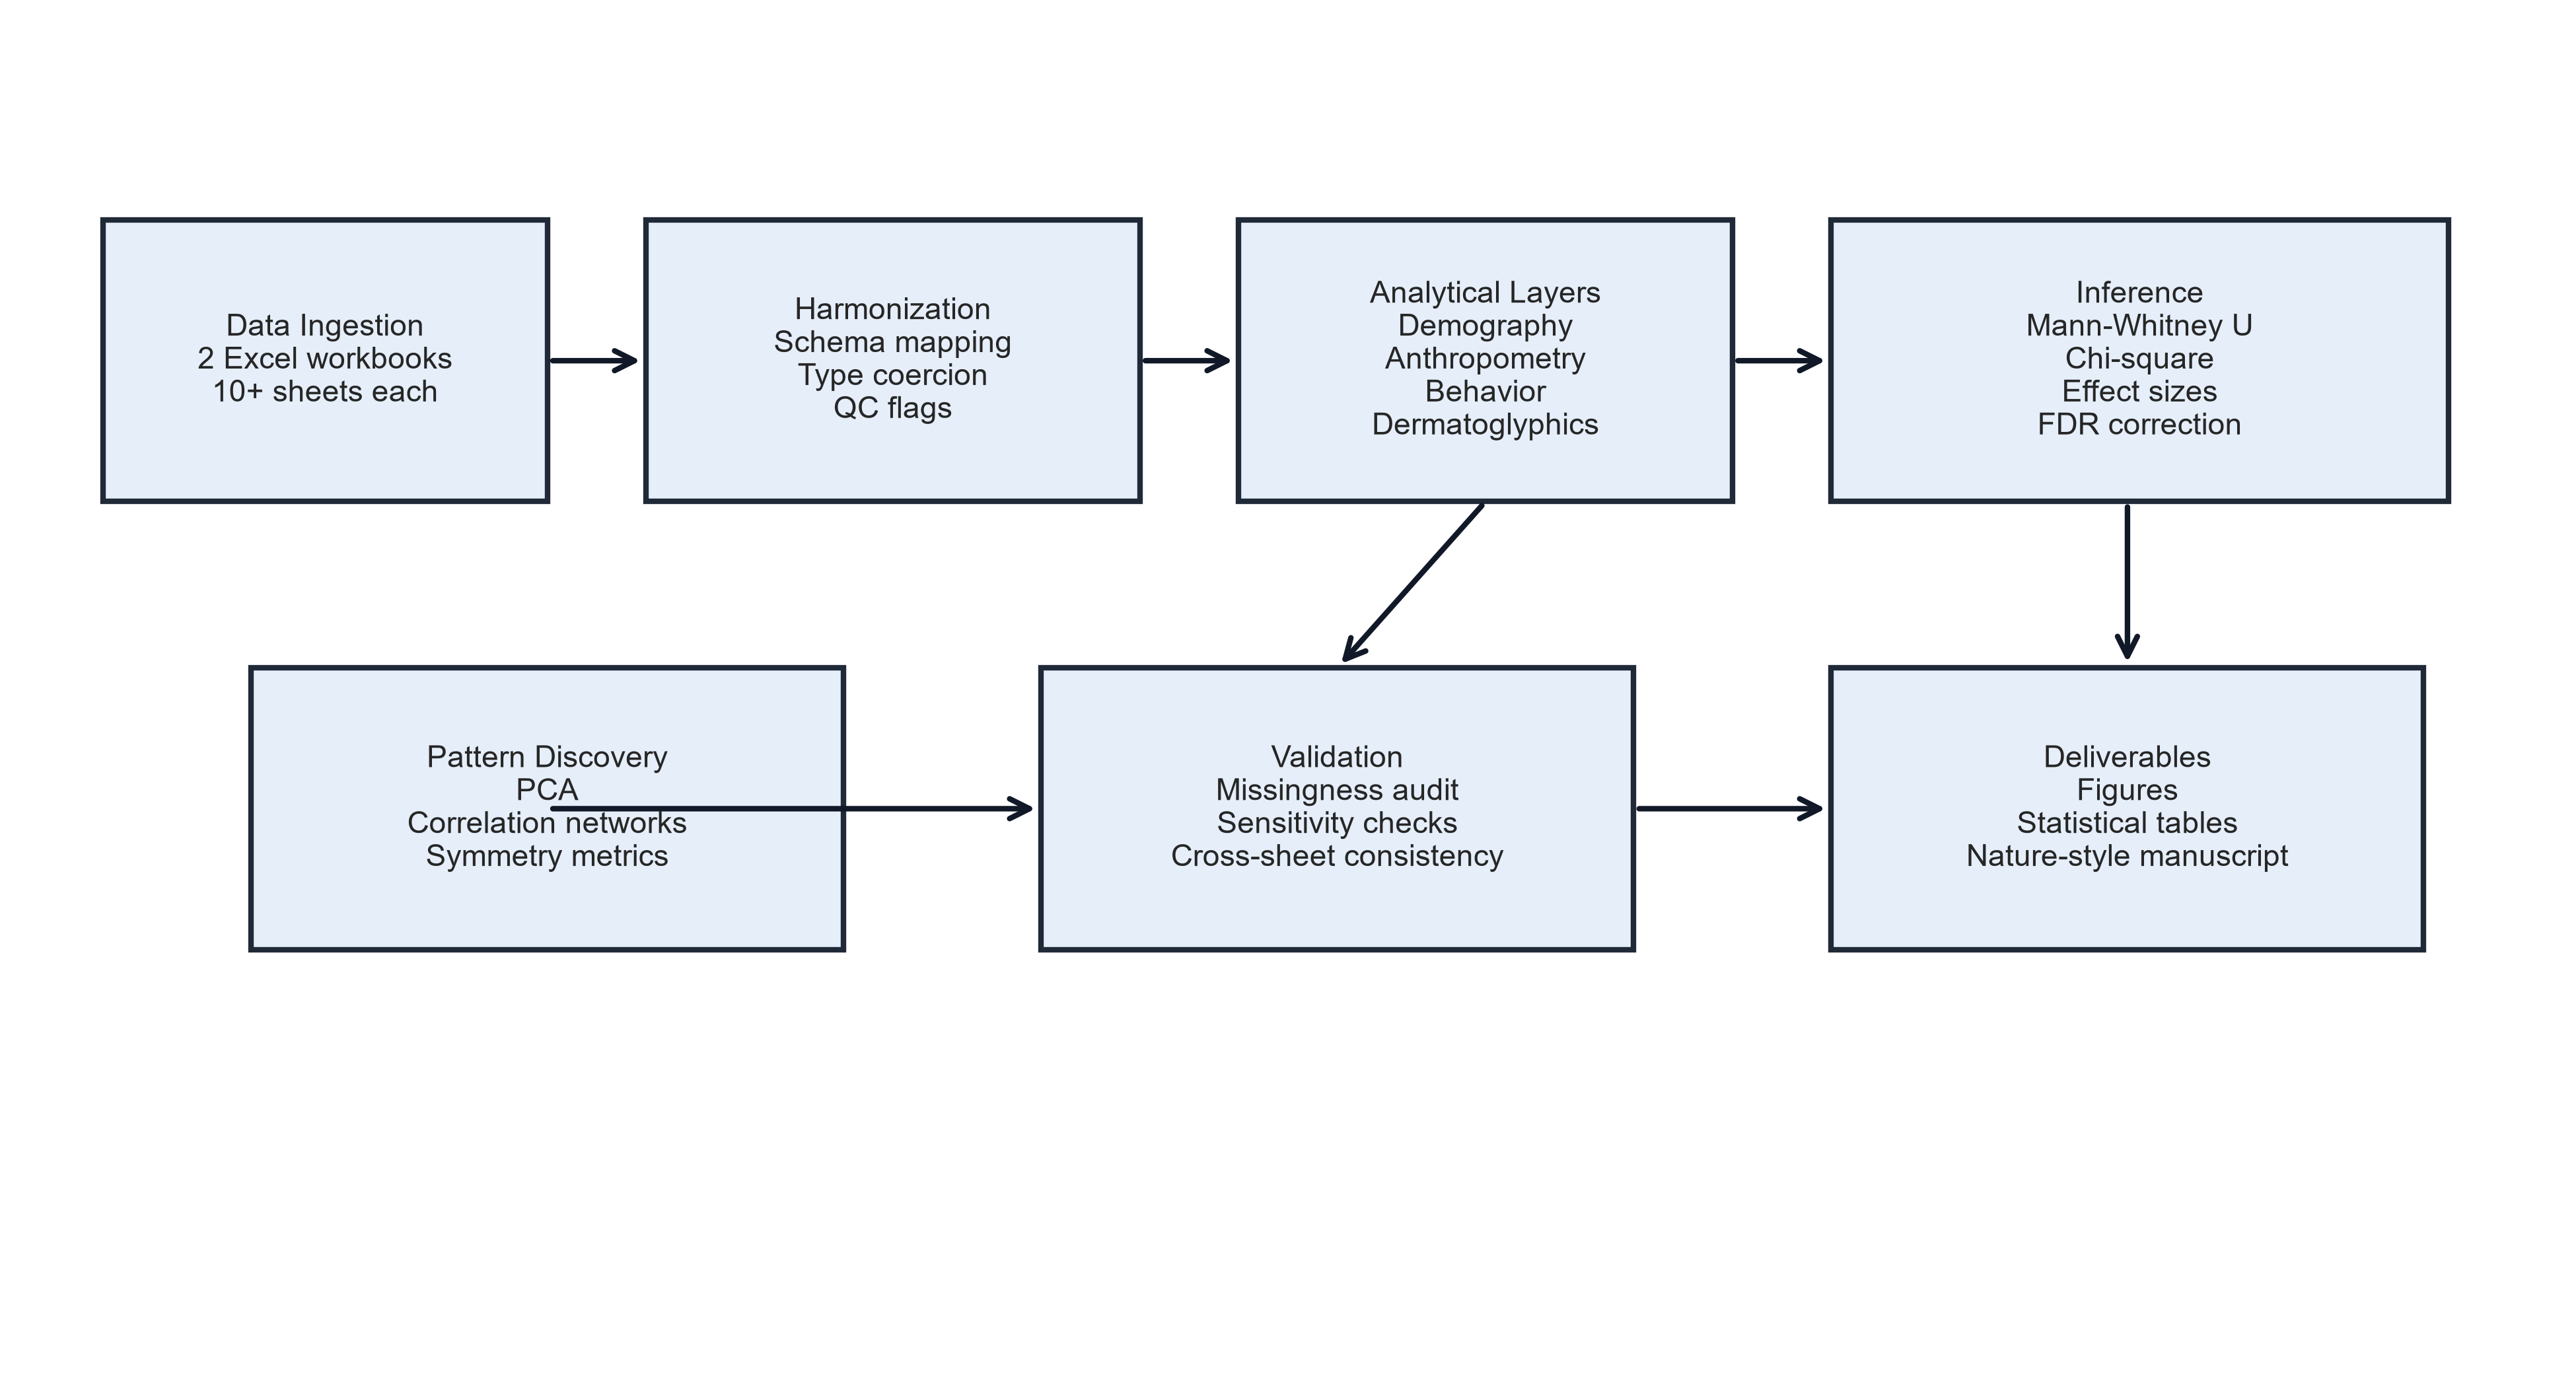
\includegraphics[width=0.95\textwidth]{figures/methodology_pipeline.png}
\caption{End-to-end methodology pipeline.}
\end{figure}

\section{Results}
\subsection{Cohort structure}
Combined roster size was 188 individuals: 120 in Nirankal and 68 in Virnoda. Median age was similar (17 vs 18 years), although the age spread was wider in Nirankal. Age-sex banding showed stronger early-age female concentration in Nirankal and a more balanced younger structure in Virnoda.

\begin{table}[H]
\centering
\caption{Cohort profile by tribe.}
\begin{tabular}{lrrrrr}
\toprule
Tribe & Roster $n$ & Male & Female & Median age & Age IQR \\
\midrule
Nirankal & 120 & 56 & 64 & 17.0 & 29.0 \\
Virnoda & 68 & 36 & 32 & 18.0 & 20.0 \\
\bottomrule
\end{tabular}
\end{table}

\begin{figure}[H]
\centering
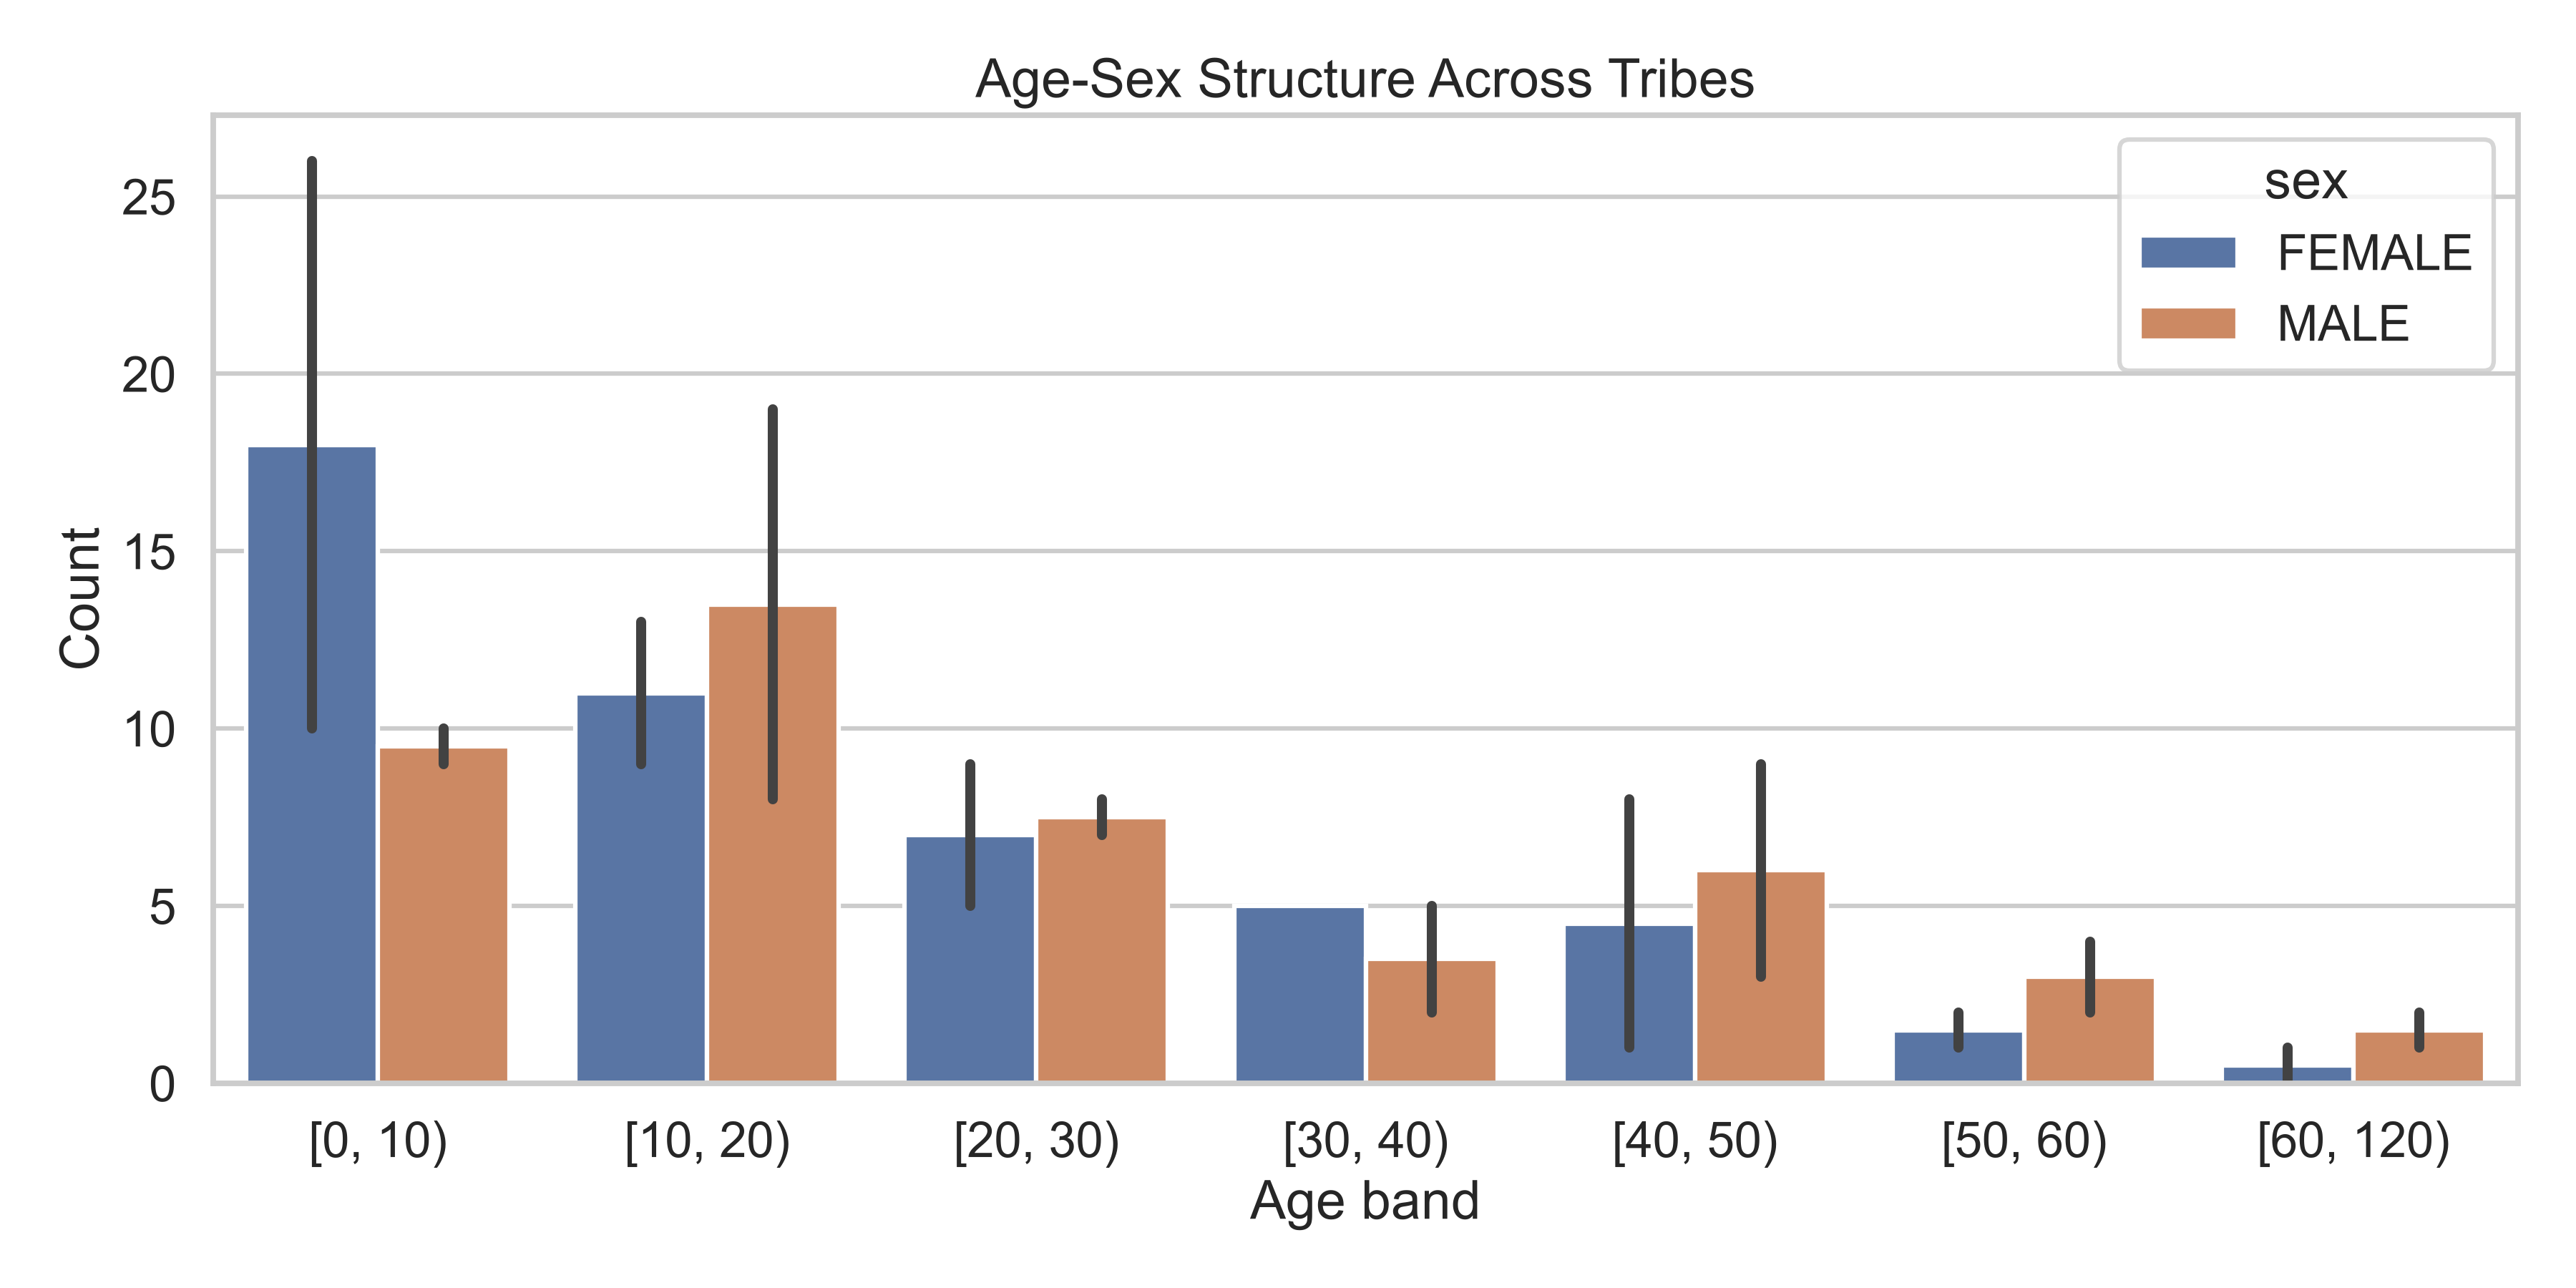
\includegraphics[width=0.9\textwidth]{figures/age_sex_structure.png}
\caption{Age-sex structure across tribes.}
\end{figure}

\subsection{Anthropometric contrasts}
Anthropometric medians were generally higher in Virnoda across BMI and most circumference variables, but standardized shifts were mostly small. The strongest nominal contrast was for biceps thickness (	extit{p}=0.021, unadjusted), though it did not remain significant after FDR correction. Figure~\ref{fig:effect} and Figure~\ref{fig:bmi} show the effect-size profile and BMI distributions.

\begin{table}[H]
\centering
\caption{Anthropometric two-sample inference and effect sizes.}
\scriptsize
\begin{tabular}{lrrrrrr}
\toprule
Variable & Median (Nir) & Median (Vir) & $p$ & $q_{BH}$ & Cohen's $d$ & Cliff's $\delta$ \\
\midrule
Biceps (mm) & 27.4 & 22.0 & 0.0213 & 0.2342 & -0.364 & 0.255 \\
BMI & 15.95 & 17.60 & 0.0936 & 0.4009 & 0.269 & -0.225 \\
Height (cm) & 139.45 & 146.51 & 0.2651 & 0.4009 & 0.137 & -0.124 \\
Waist Cir (cm) & 58.30 & 62.00 & 0.2967 & 0.4009 & 0.207 & -0.116 \\
Weight (kg) & 33.29 & 38.10 & 0.3024 & 0.4009 & 0.231 & -0.114 \\
Hip Cir (cm) & 70.39 & 77.20 & 0.3149 & 0.4009 & 0.236 & -0.111 \\
Head Cir (cm) & 50.39 & 50.00 & 0.9338 & 0.9592 & 0.017 & 0.010 \\
\bottomrule
\end{tabular}
\end{table}

\begin{figure}[H]
\centering
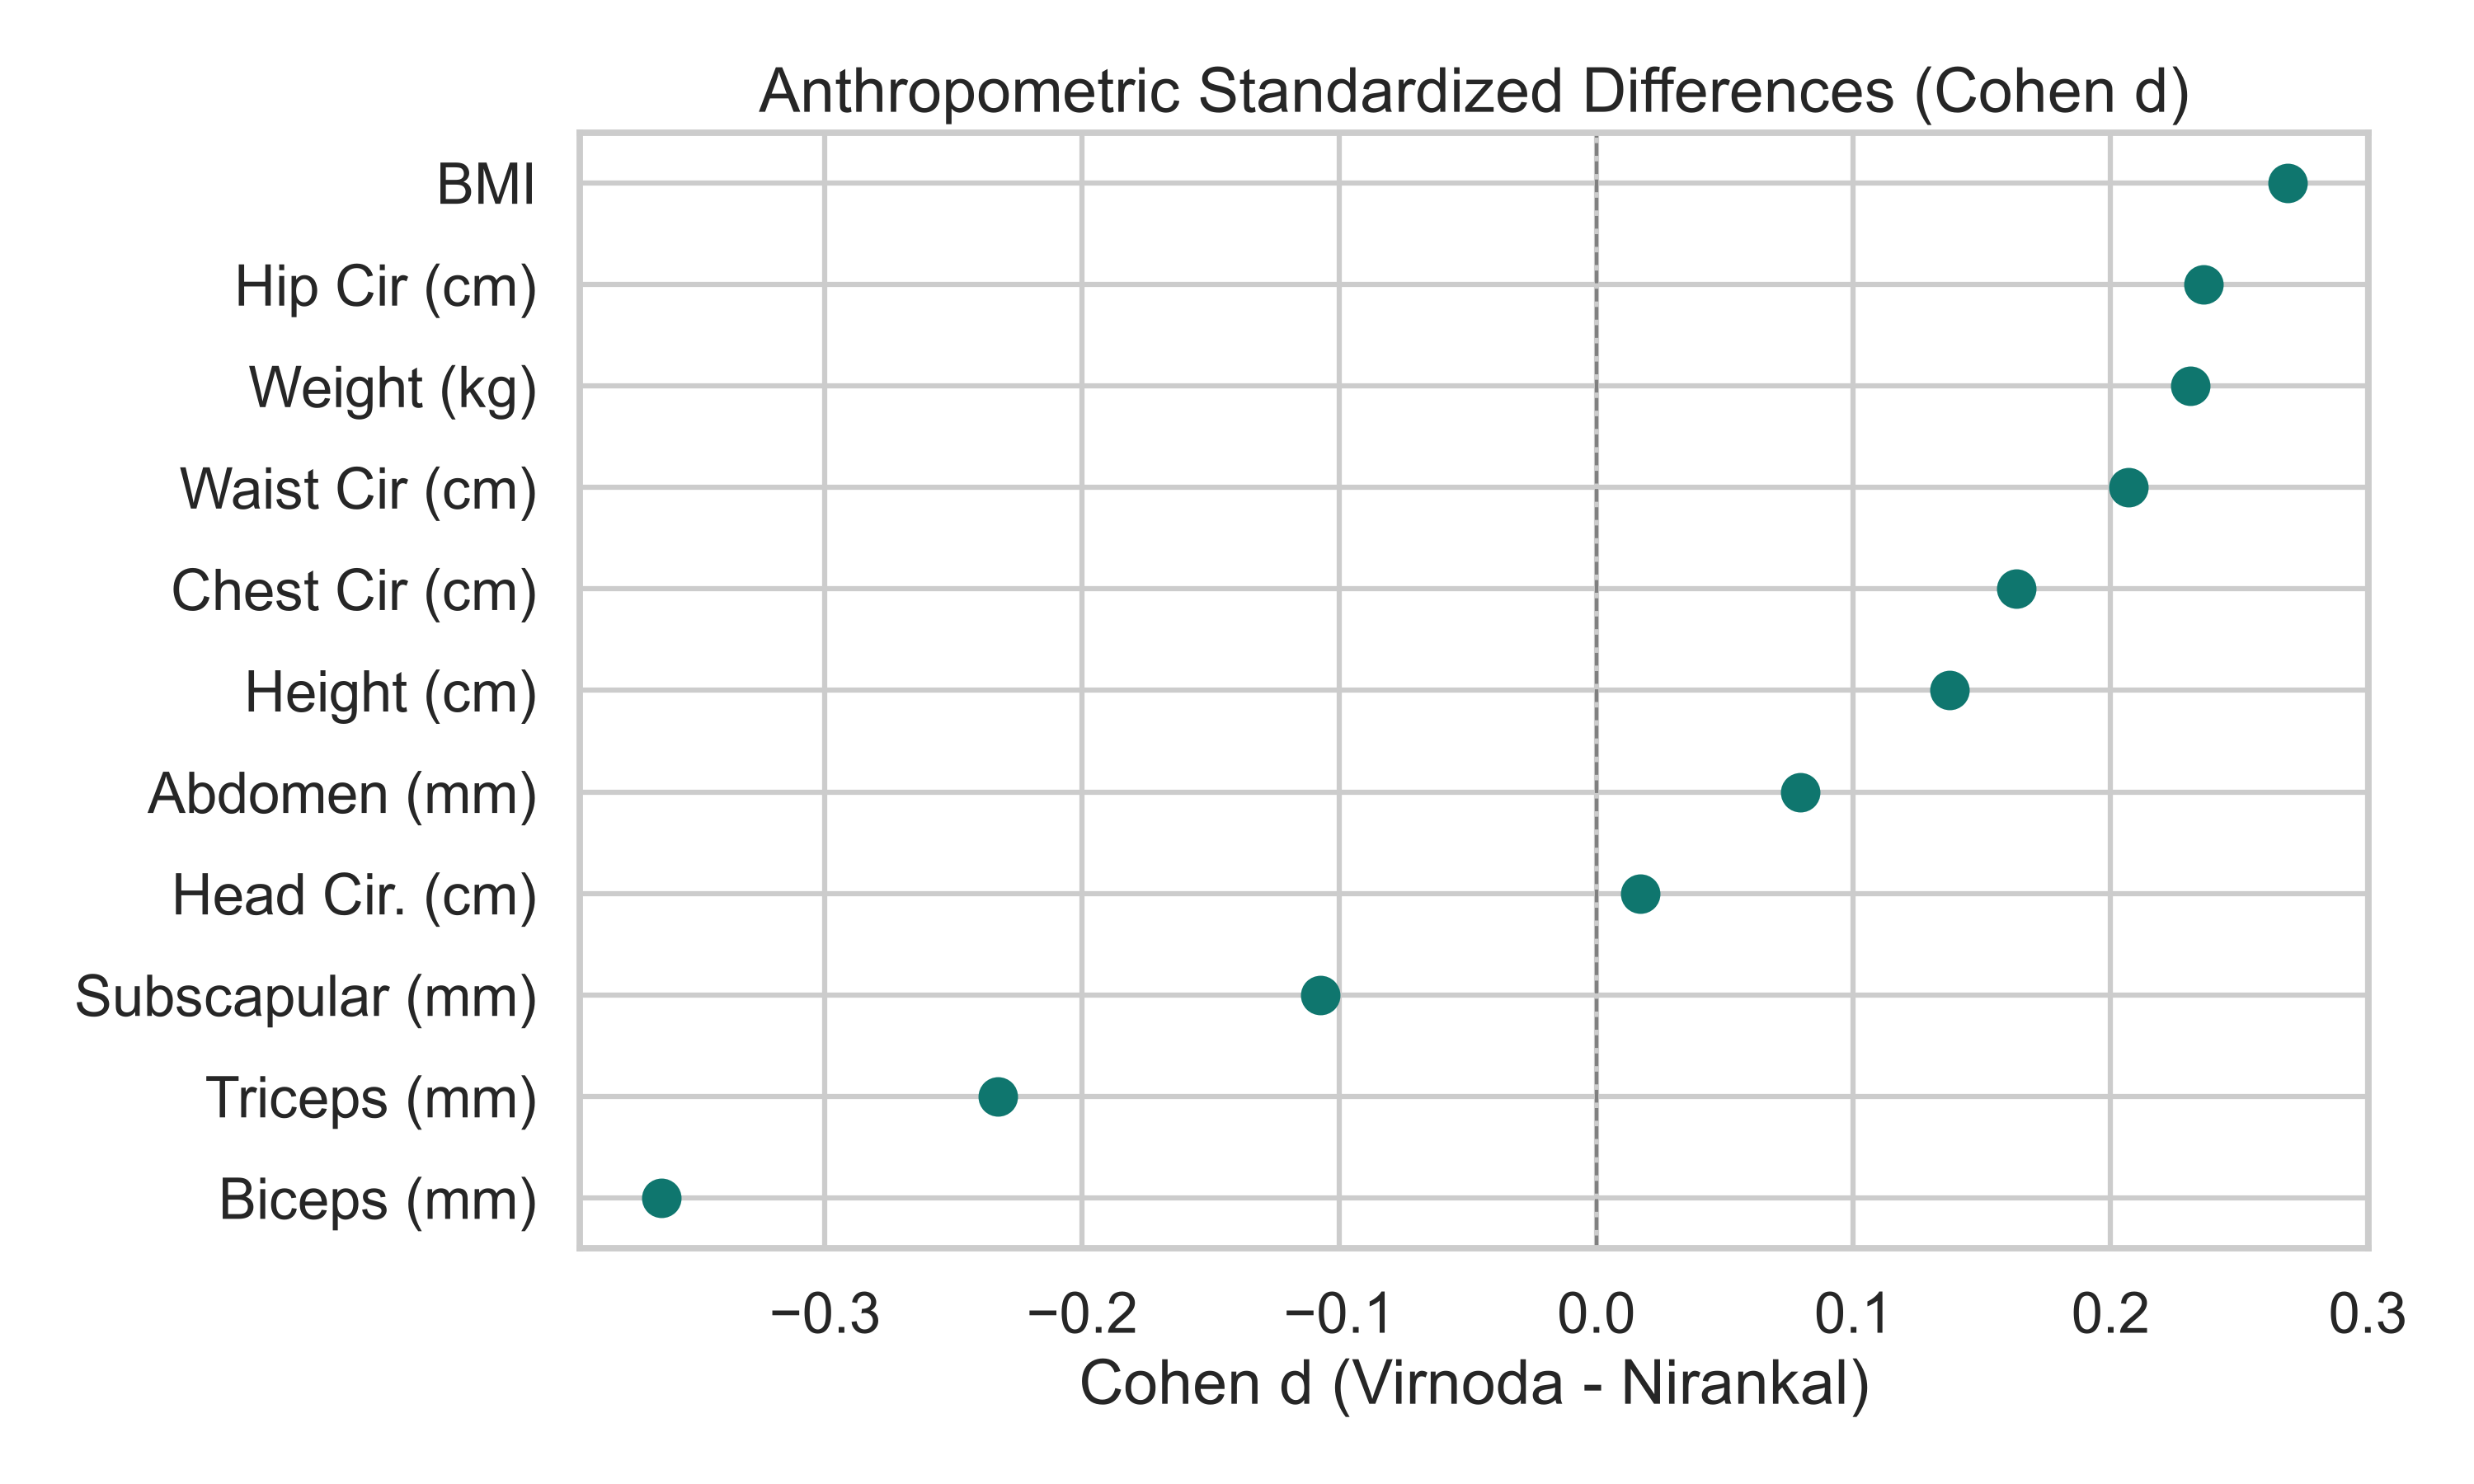
\includegraphics[width=0.85\textwidth]{figures/effect_sizes_cohens_d.png}
\caption{Anthropometric standardized differences (Cohen's $d$).}
\label{fig:effect}
\end{figure}

\begin{figure}[H]
\centering
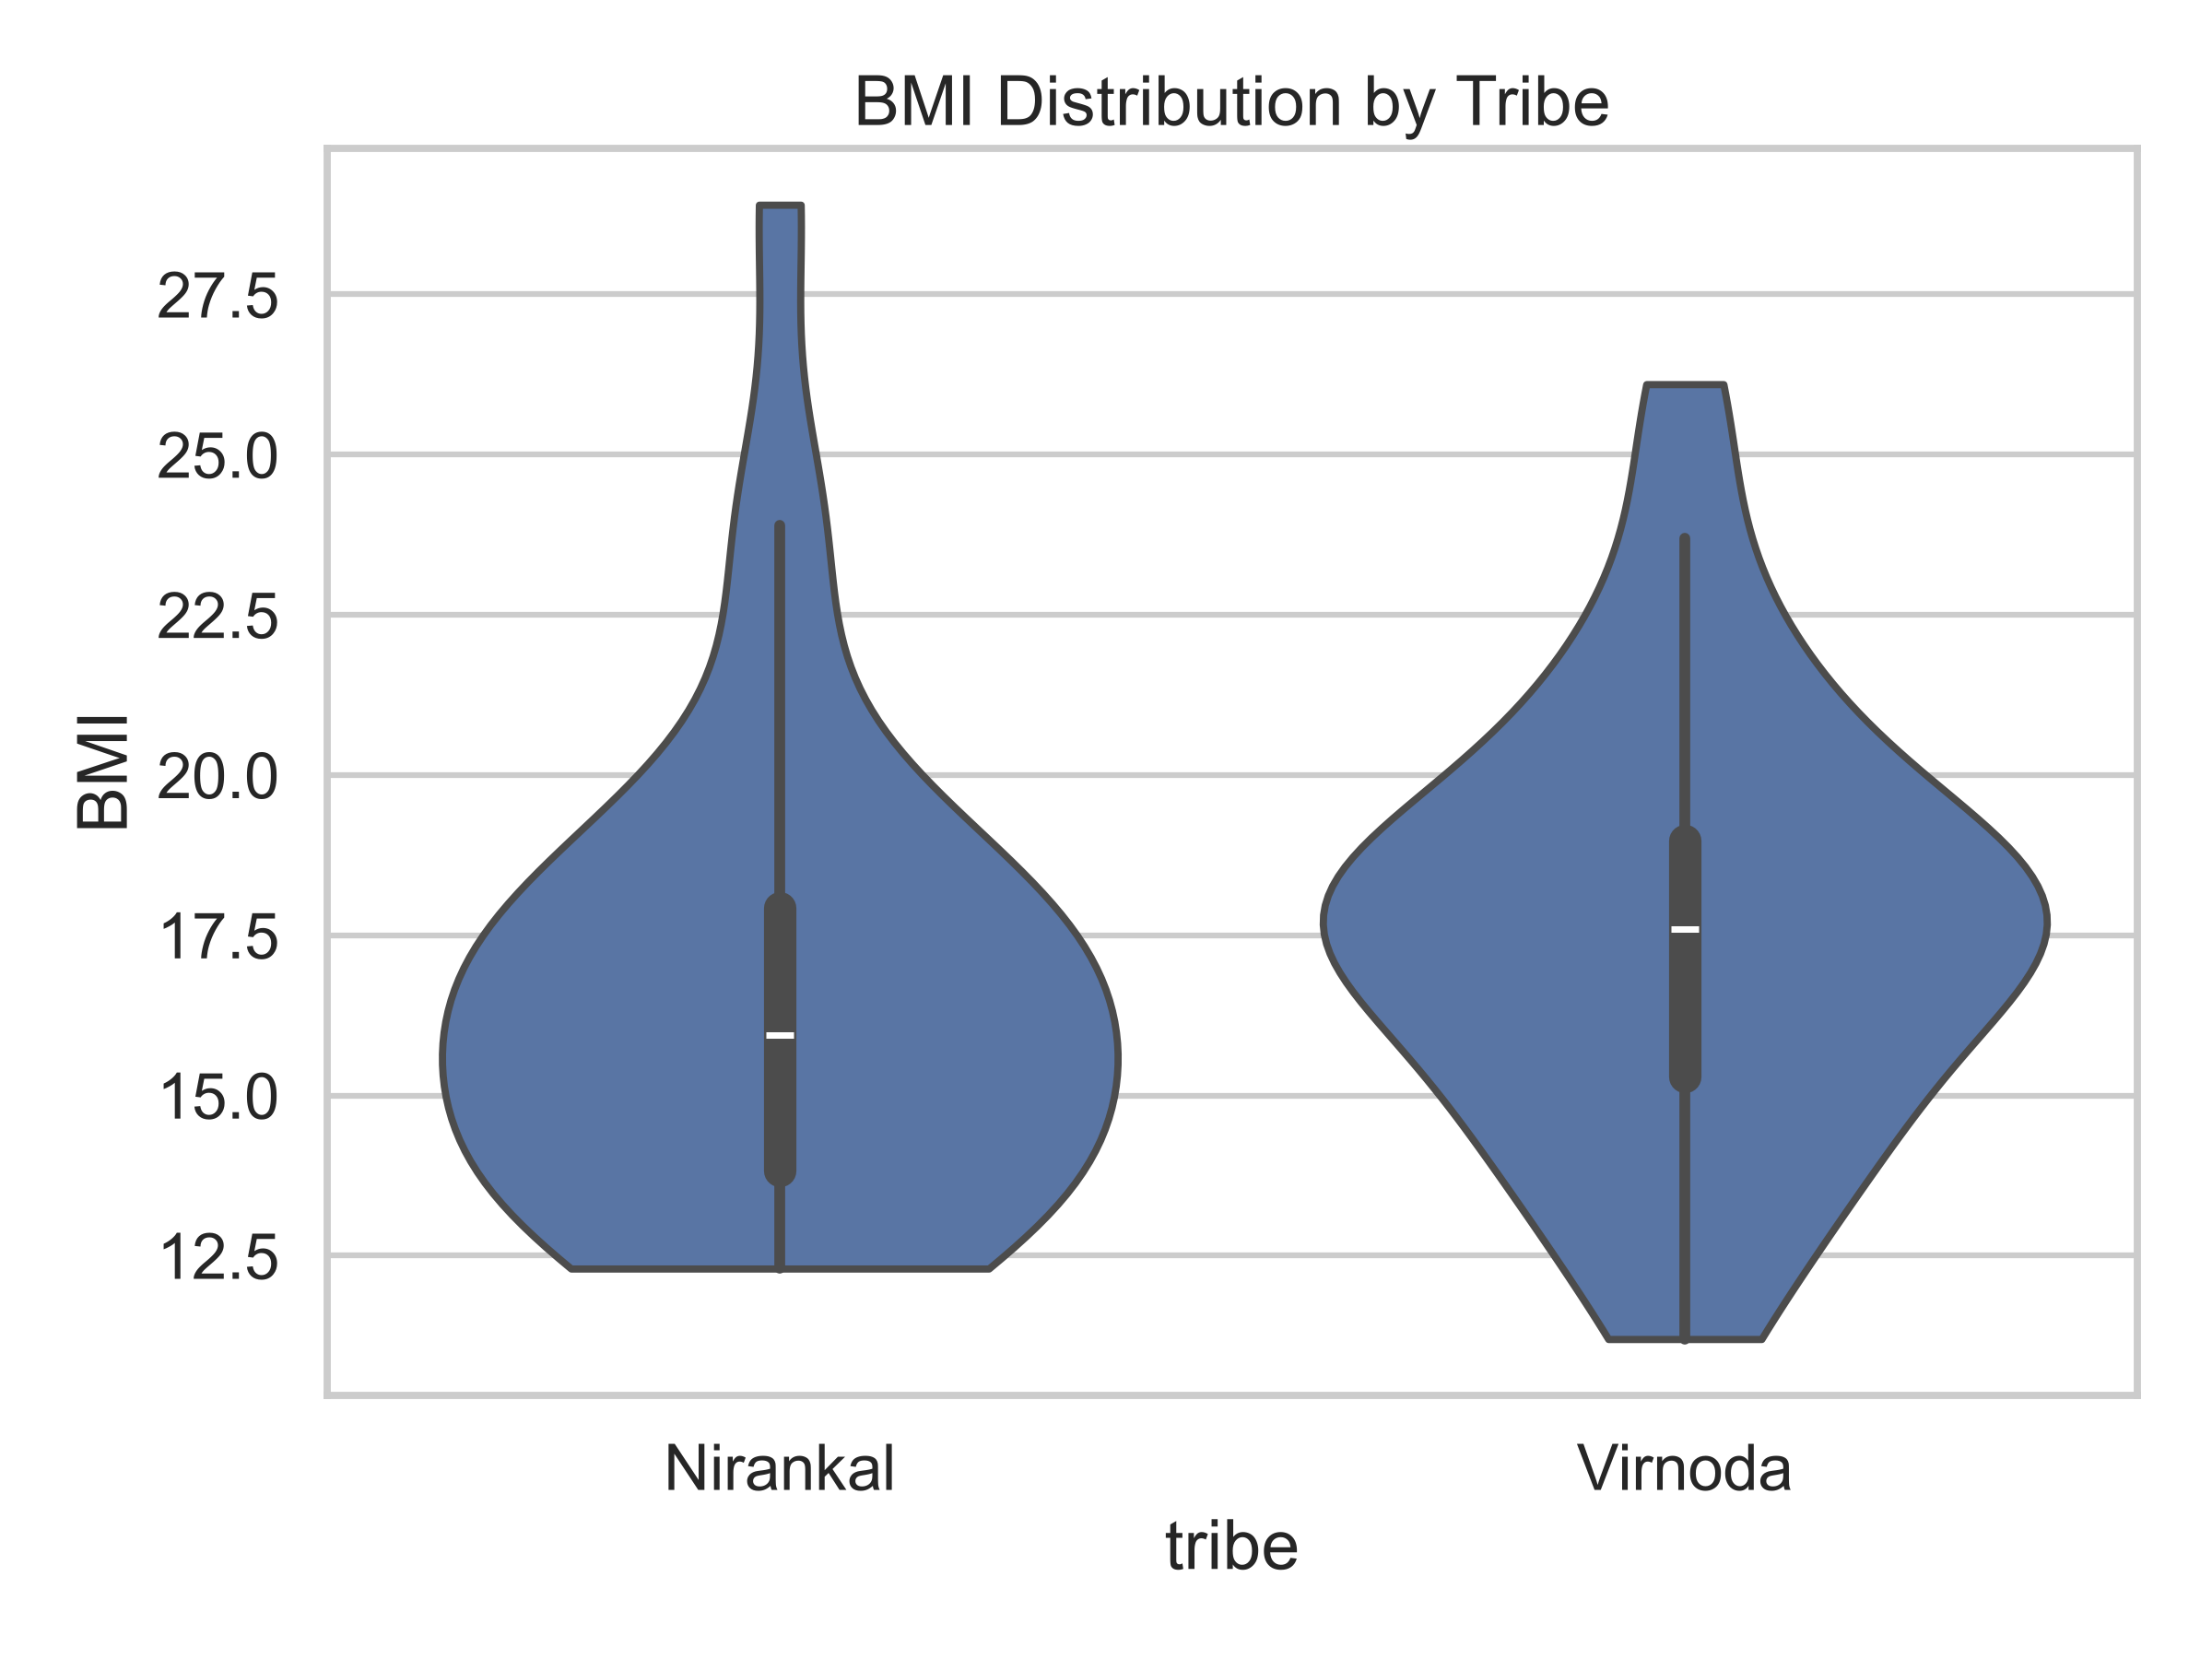
\includegraphics[width=0.7\textwidth]{figures/bmi_violin.png}
\caption{BMI distribution by tribe.}
\label{fig:bmi}
\end{figure}

\subsection{Behavioral and socioeconomic structure}
Questionnaire structure differed most in work and tobacco categories. Main-work responses showed the strongest categorical divergence, and tobacco-use divergence was also prominent. Non-never exposure rates were higher in Virnoda for tobacco and alcohol-related responses.

\begin{figure}[H]
\centering
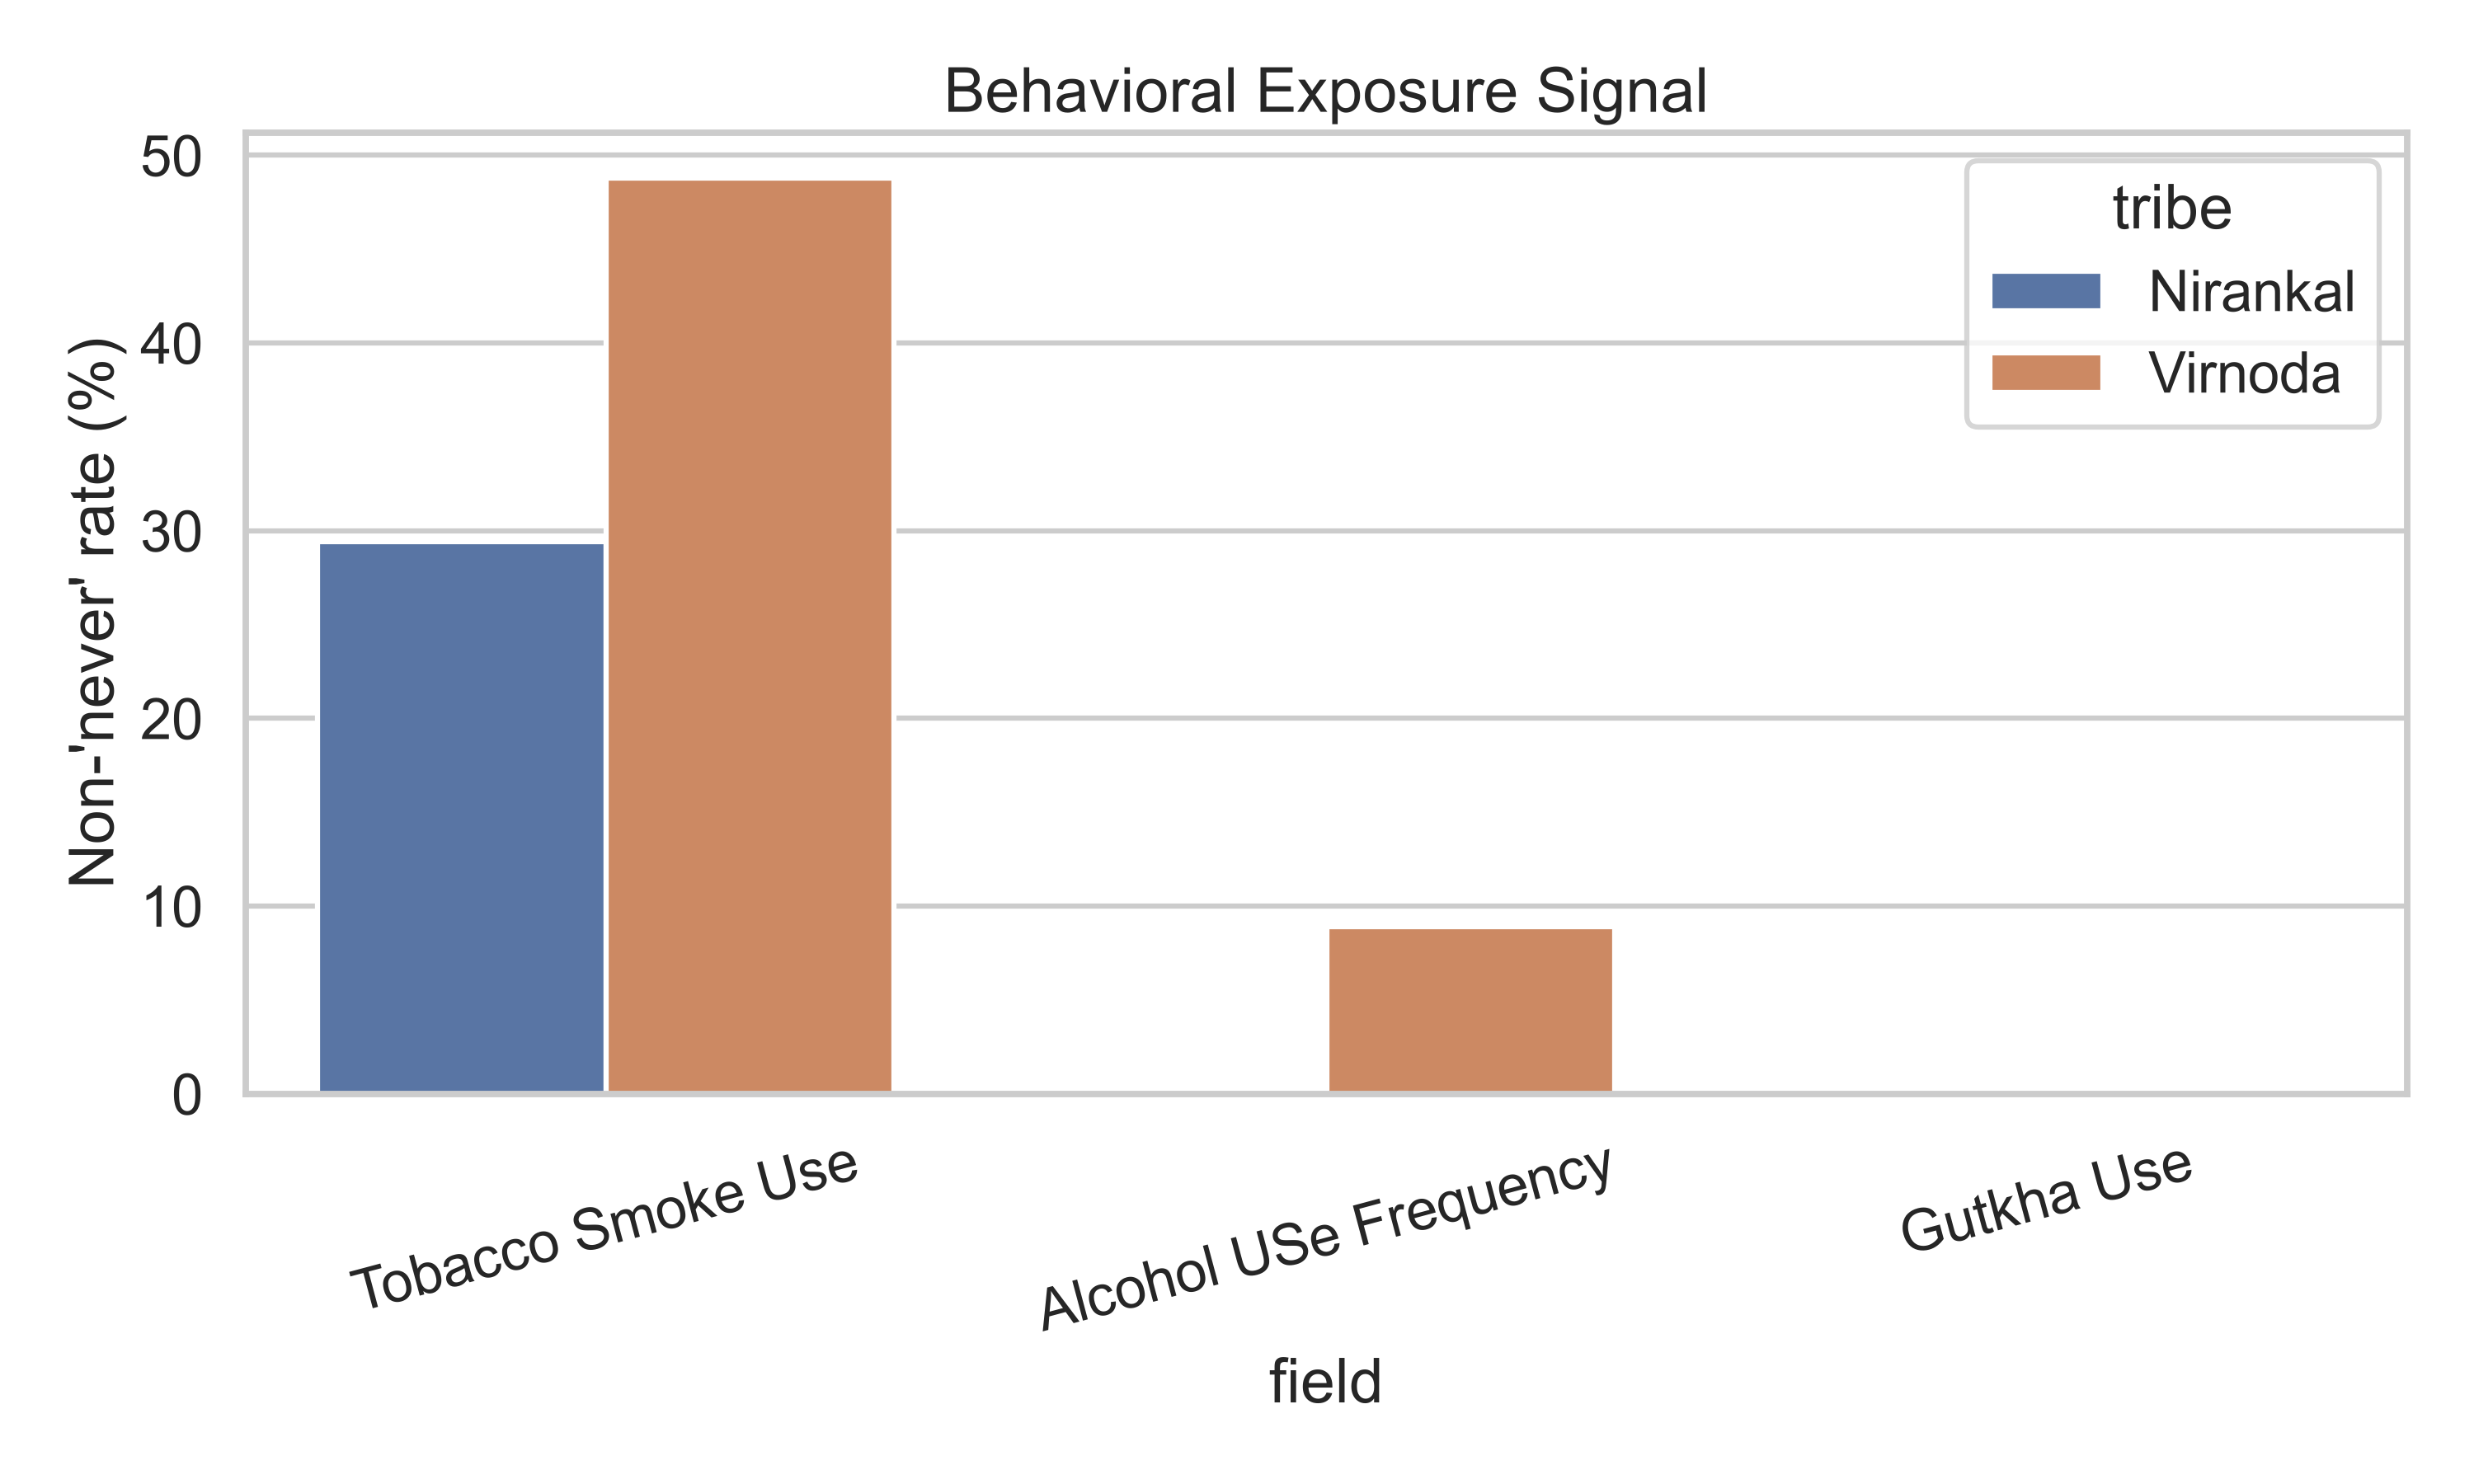
\includegraphics[width=0.9\textwidth]{figures/behavior_non_never_rates.png}
\caption{Behavioral exposure signal represented as non-never response rates.}
\end{figure}

\subsection{Dermatoglyphic composition}
Both tribes shared dominant fingerprint code classes (W, UL, PA), but composition and diversity differed. Nirankal displayed a broader repertoire (58 unique normalized codes; Shannon entropy 3.205), whereas Virnoda was more concentrated (7 unique codes; entropy 2.179). Fingerprint symmetry showed broadly similar left-right match rates, with some finger-level divergence.

\begin{figure}[H]
\centering
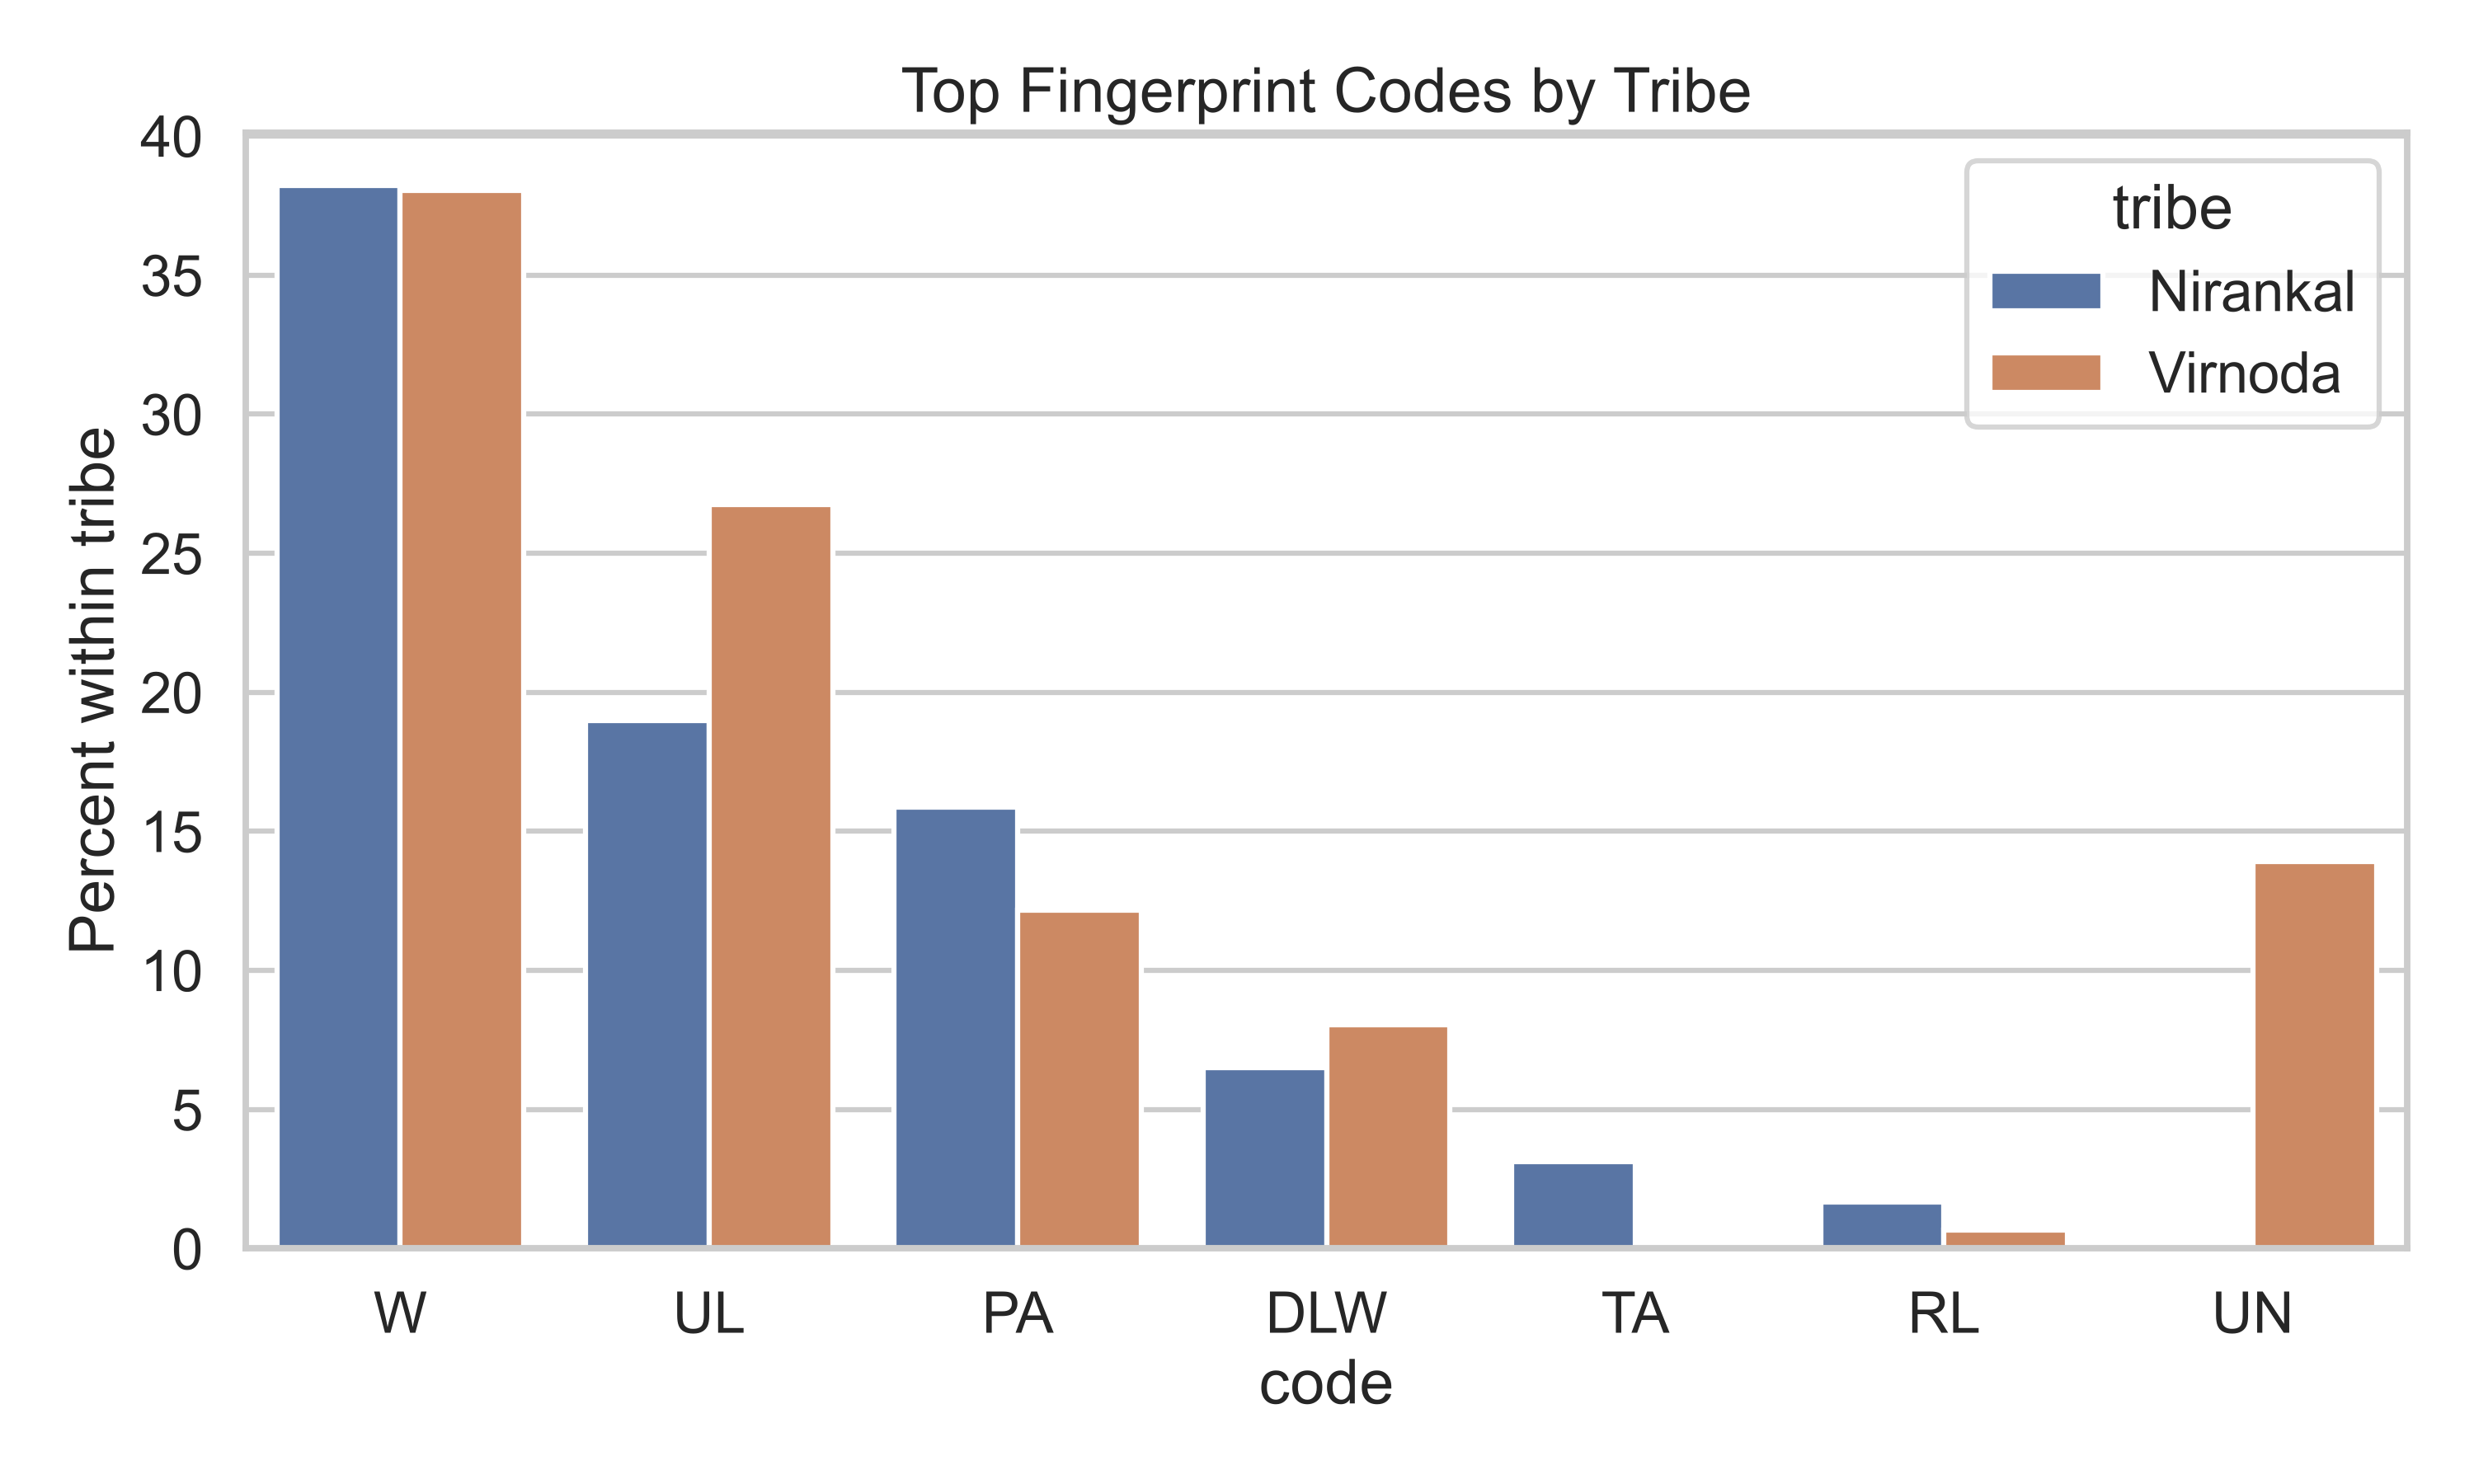
\includegraphics[width=0.85\textwidth]{figures/fingerprint_top_codes.png}
\caption{Top fingerprint code composition by tribe.}
\end{figure}

\begin{figure}[H]
\centering
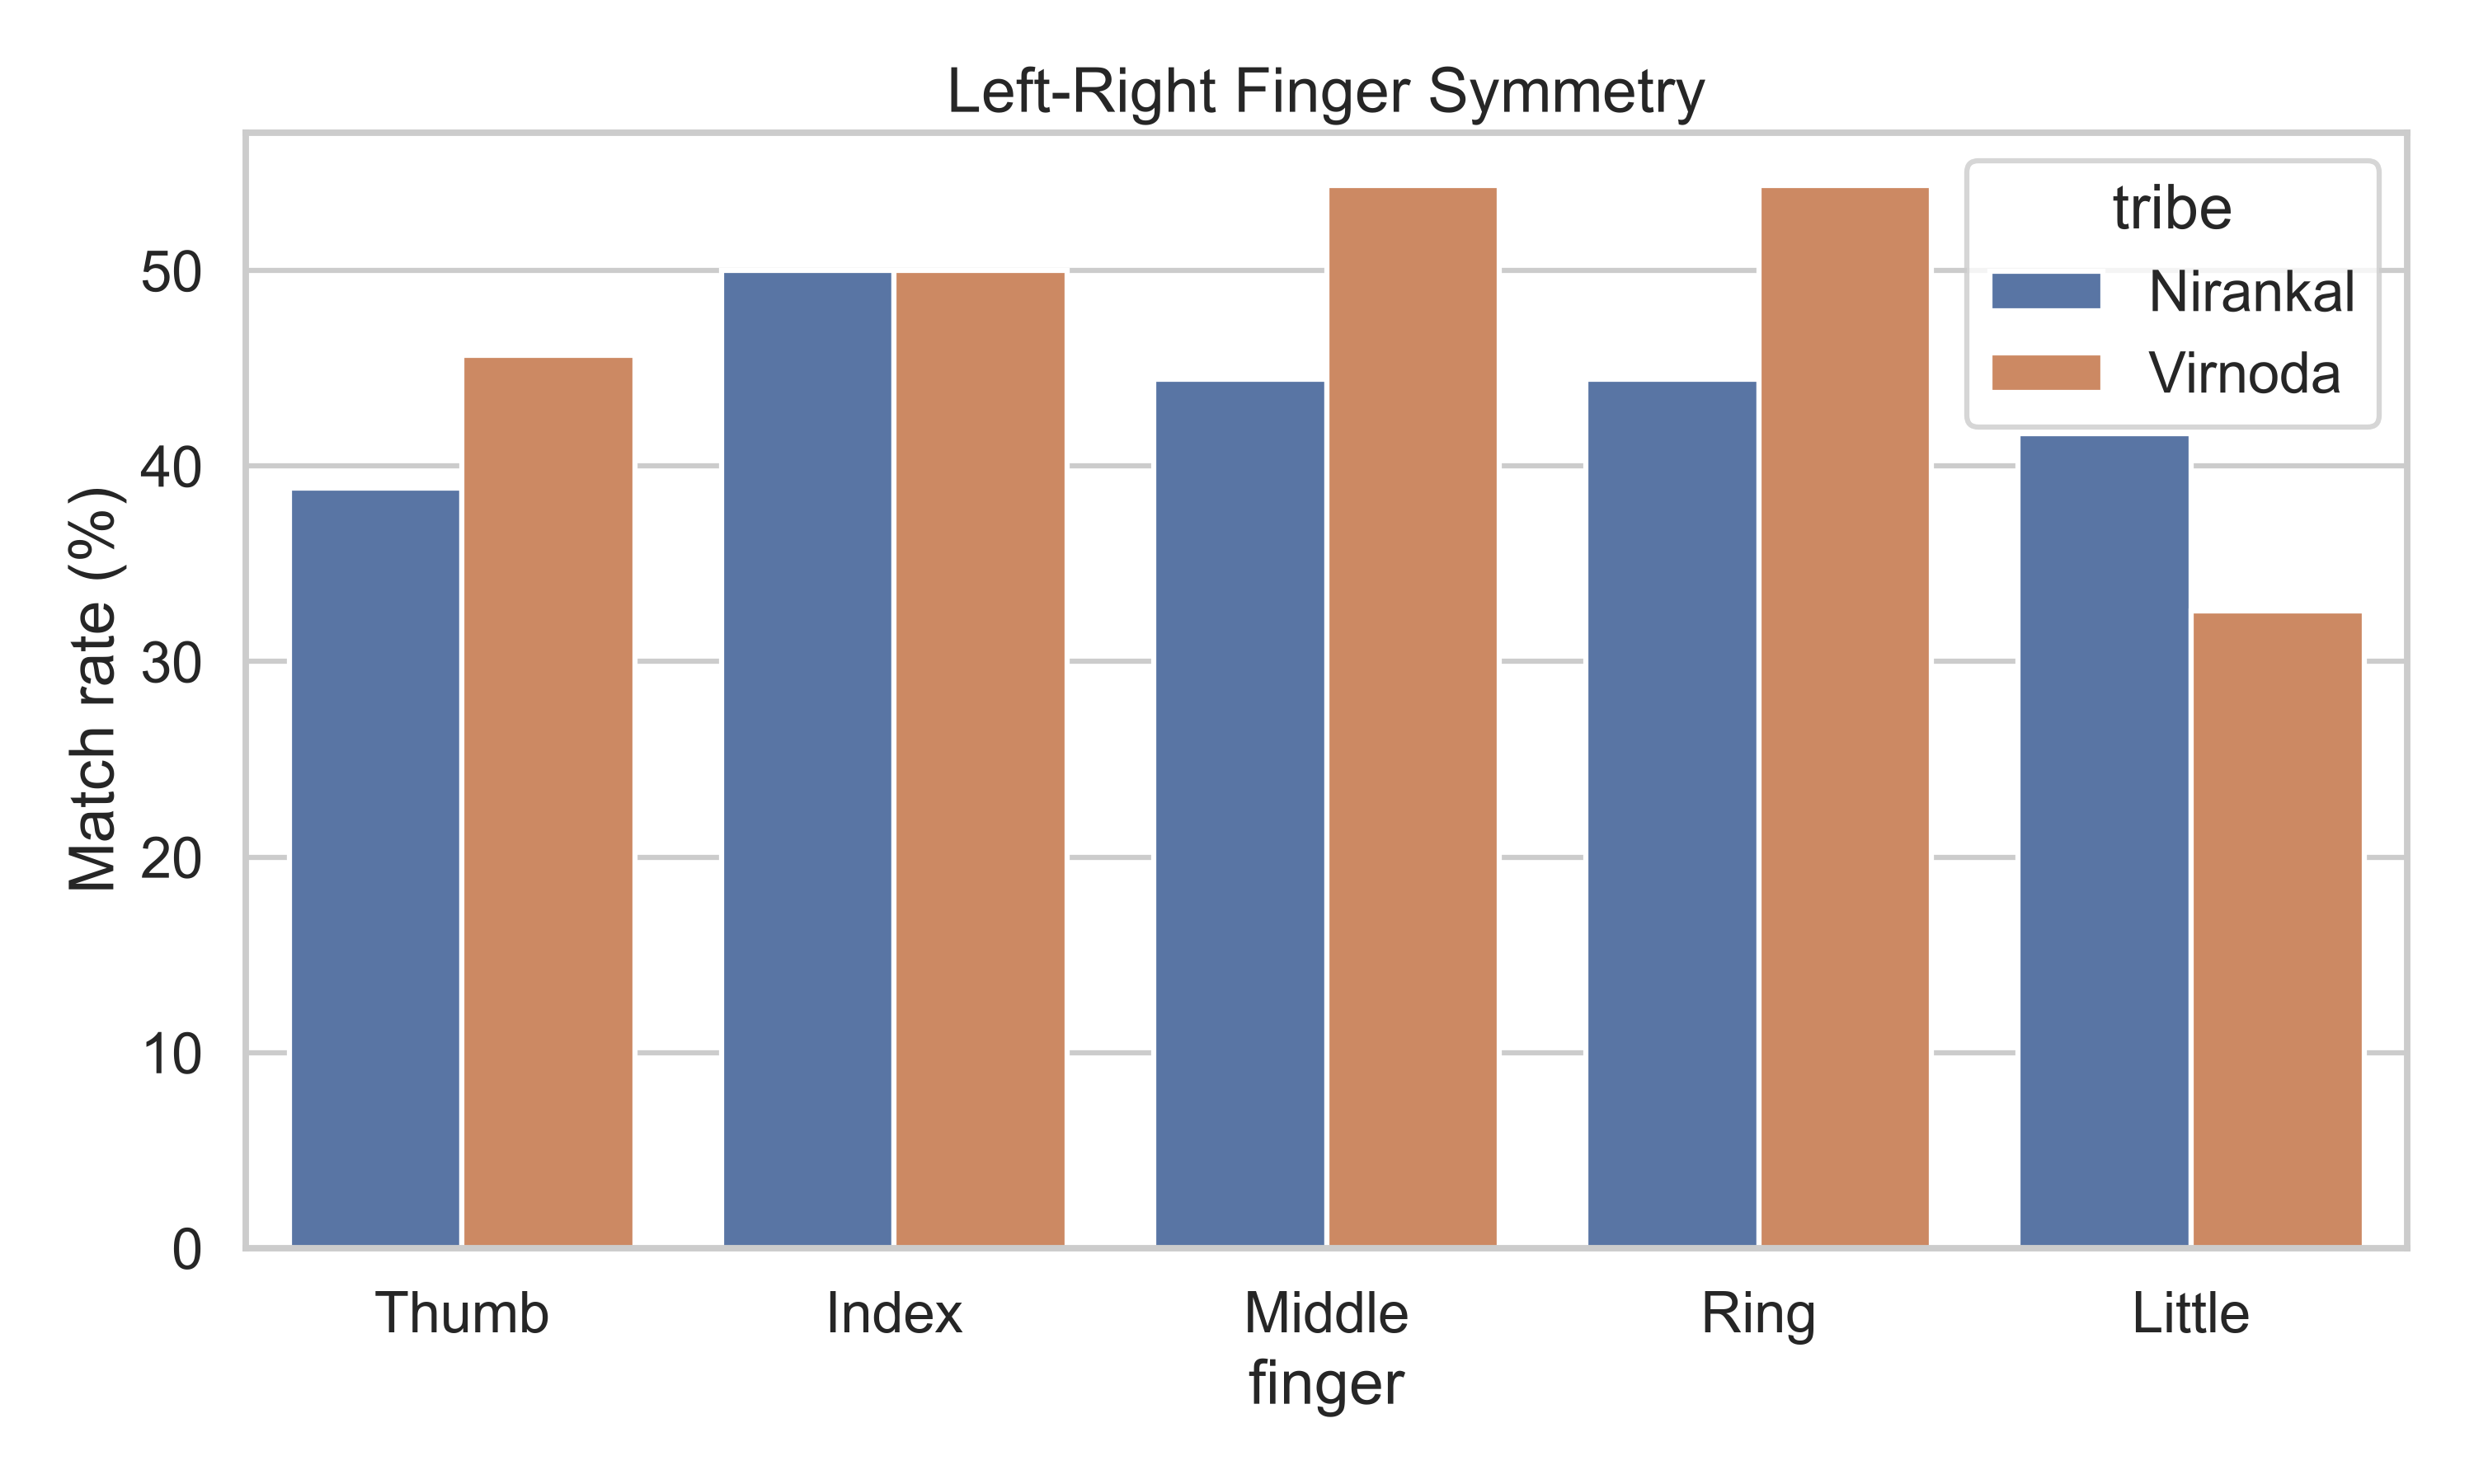
\includegraphics[width=0.85\textwidth]{figures/fingerprint_symmetry.png}
\caption{Left-right same-finger symmetry rates by tribe.}
\end{figure}

\subsection{Multivariate structure}
PCA of anthropometric variables yielded partially overlapping tribe clouds with directionally shifted centroids rather than fully separated clusters.

\begin{figure}[H]
\centering
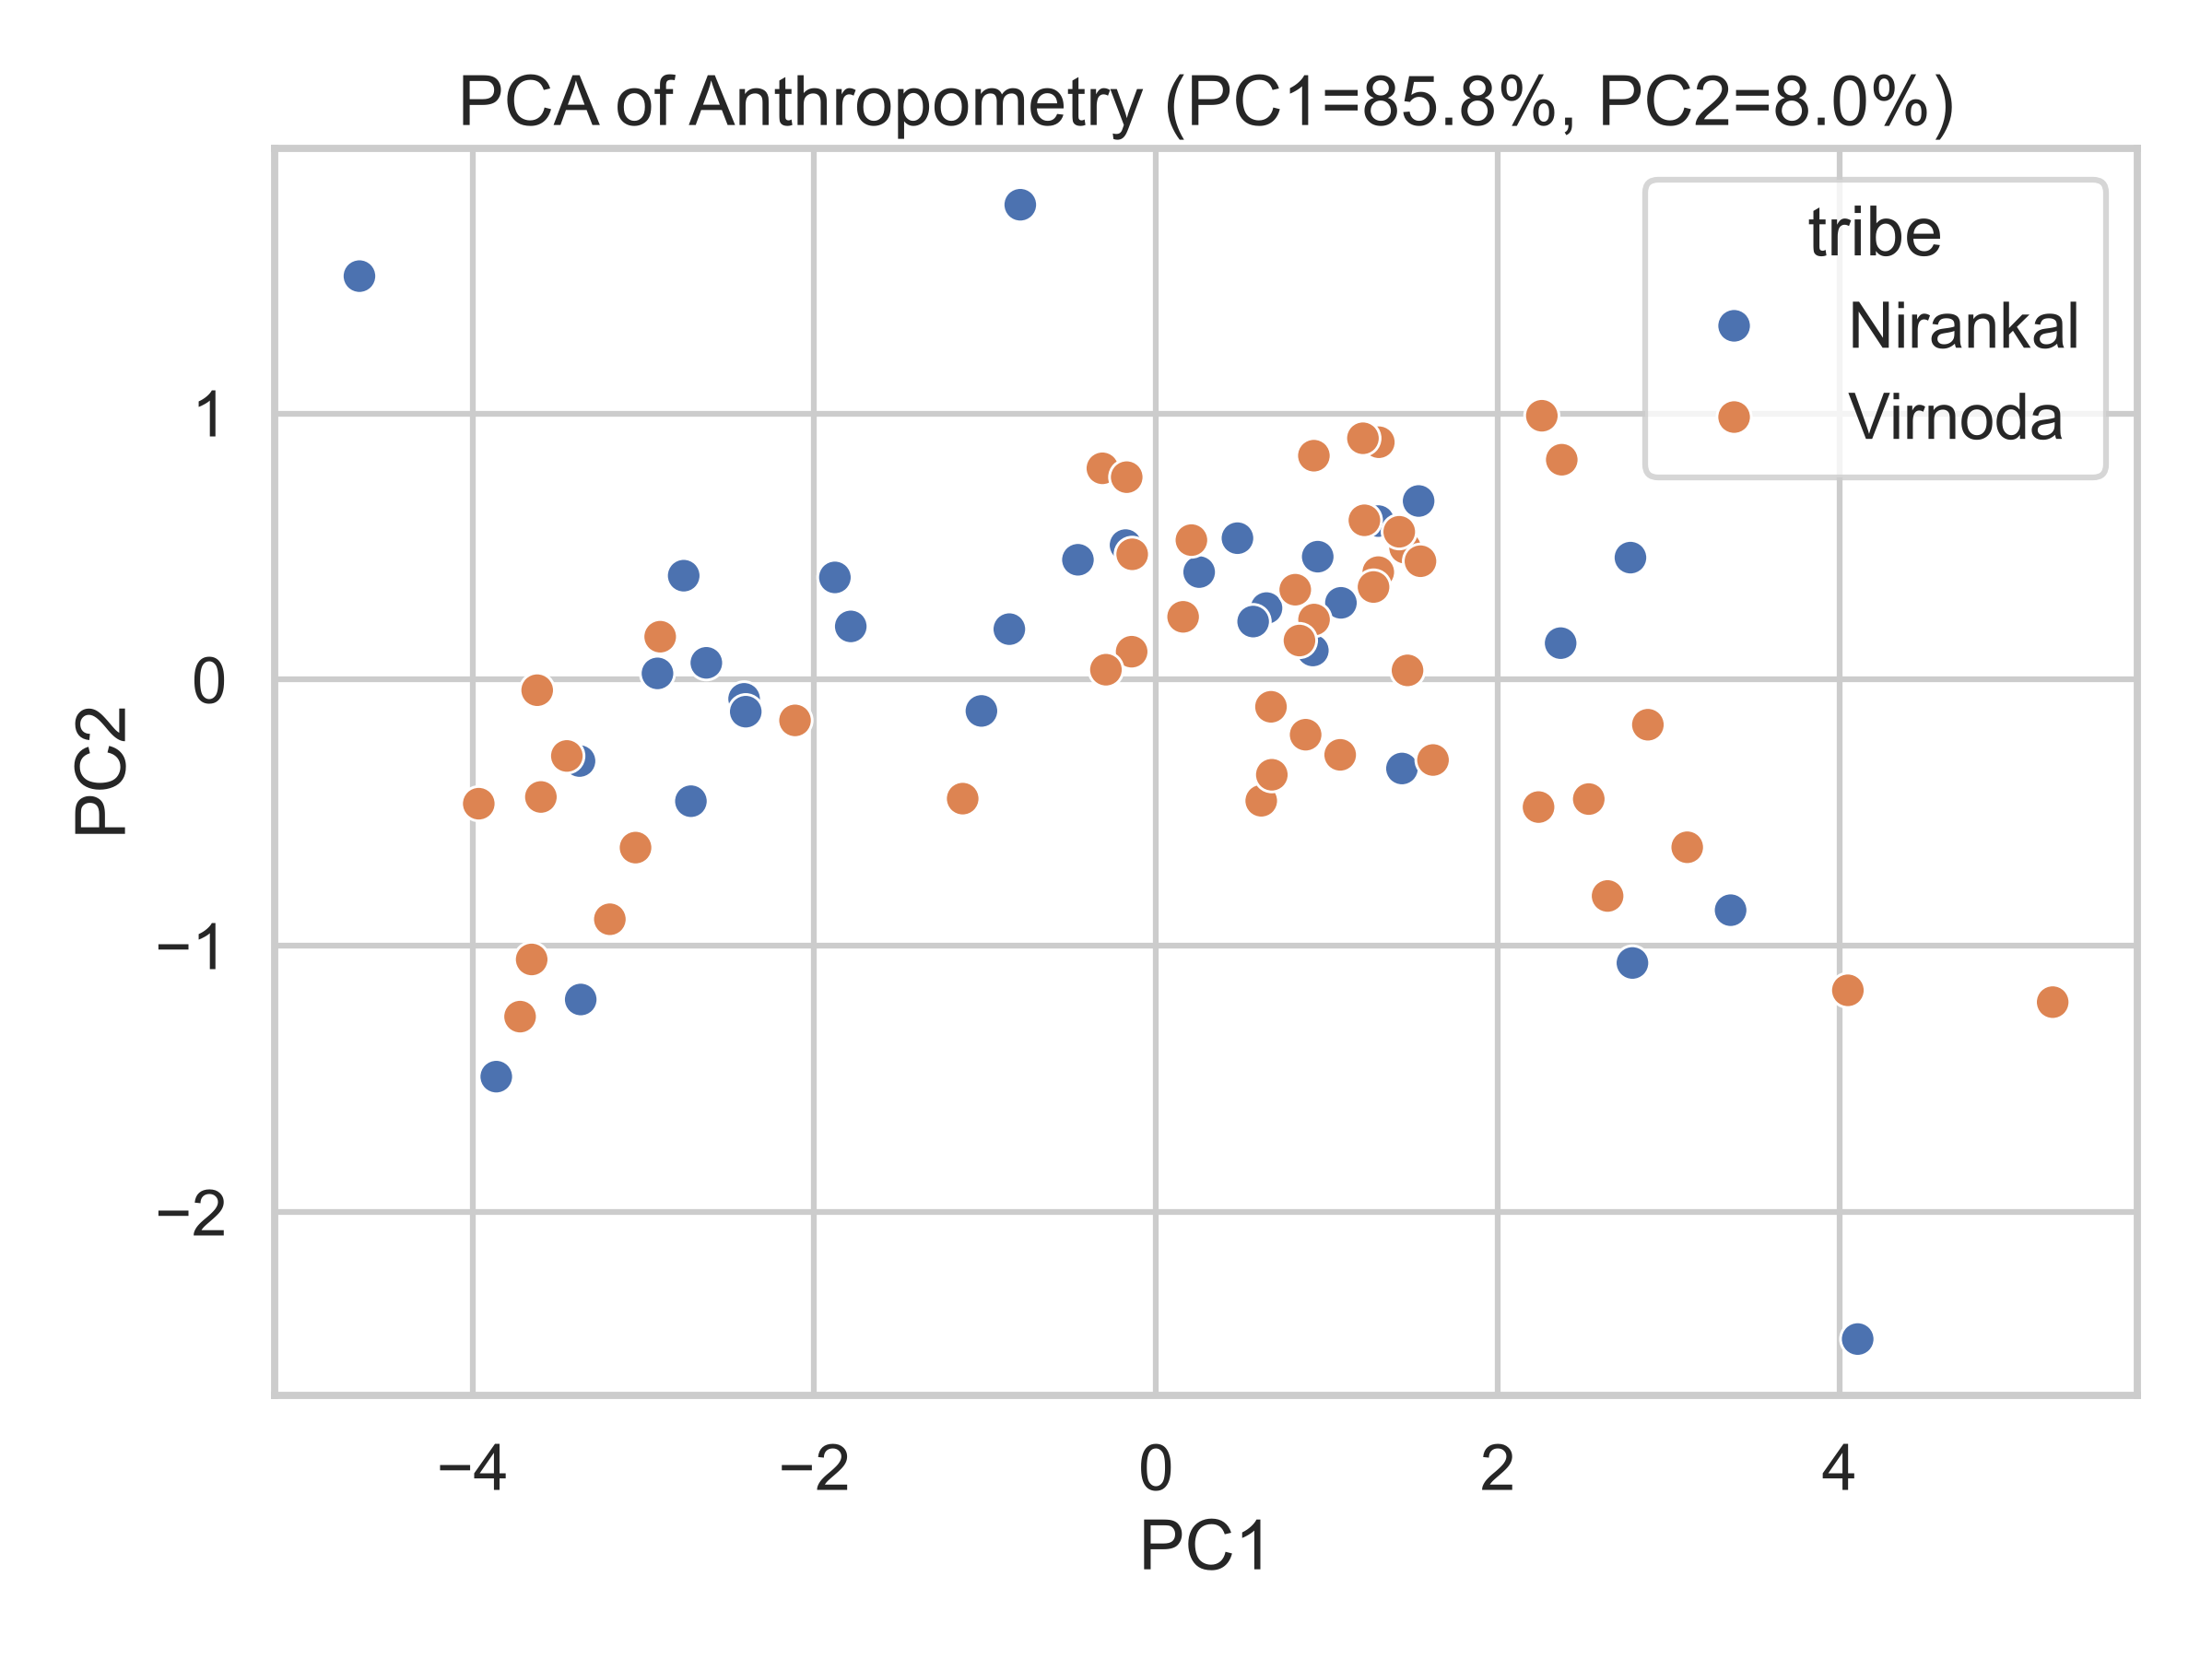
\includegraphics[width=0.75\textwidth]{figures/anthropometry_pca.png}
\caption{PCA projection of anthropometric features.}
\end{figure}

\section{Discussion}
The results indicate that cross-tribe differences are detectable but generally moderate in anthropometric magnitude, with small standardized effect sizes and substantial overlap. Behavioral patterns, especially tobacco-use responses, carry stronger discriminative signal. Dermatoglyphic diversity patterns also differ meaningfully even though dominant classes are shared. The integrated pipeline offers a reproducible template for future biosocial studies.

\section{Conclusion}
An integrated analysis of Nirankal and Virnoda data indicates that cross-tribe structure is multidimensional: demographic and anthropometric shifts are measurable but modest, behavioral responses provide stronger divergence in specific domains, and dermatoglyphic diversity patterns differ despite common dominant classes.

\section{Author contributions}
Ranji Kolkar conceived the study, curated the data schema, and supervised analysis. Swea Nidhi designed and executed the statistical pipeline, generated figures and tables, and drafted the manuscript. Both authors interpreted results and approved the final version.

\section{Competing interests}
The authors declare no competing interests.

\bibliographystyle{plain}
\bibliography{references}

\end{document}
